\documentclass[UTF8]{ctexbeamer}
\usefonttheme{serif}
\usepackage[labelformat=empty]{caption}
% Set the theme
\usetheme{Berlin}

% title, author, date
\title{An Implementation of DVCM in Water Hammer Event}
\author{刘锦坤;姜逸轩;黑建聪}
\date{2024.5.21}

\begin{document}

% Page of title
\begin{frame}
    \titlepage
\end{frame}

% Page of content
\begin{frame}{Outline}
    \tableofcontents
\end{frame}

\section{Introduction of DVCM}

\begin{frame}{Introduction of DVCM}
    \begin{figure}
        \centering
        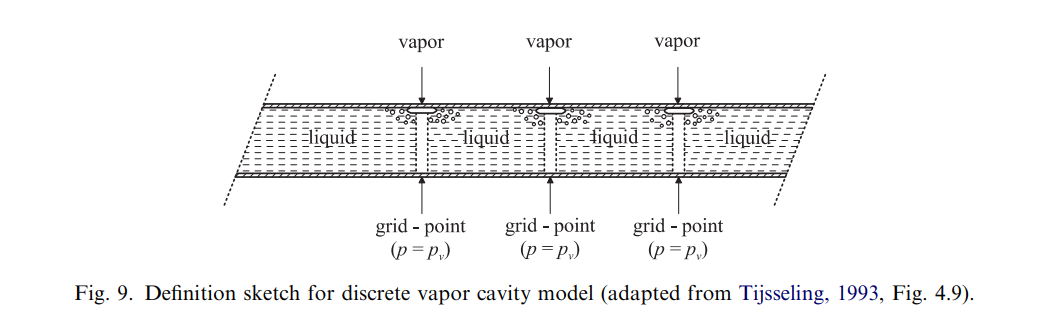
\includegraphics[width=0.8\textwidth]{pic/DVCM_Model.png}
        \caption{Sketch of DVCM Model}
    \end{figure}
    The sketch of DVCM is shown in the figure above. The DVCM model is a 1D model that can simulate the water hammer event in the pipeline. The model allows the discrete cavitation bubbles to be generated and collapsed at the grid points.
\end{frame}

\section{Details of DVCM}

\begin{frame}{Details of DVCM}
    The basic equations of MOC(method of characteristics) are farmiliar to us. The equations are shown below:
    \begin{equation}
        \begin{cases}
            H^t_j-H^{t-\Delta t}_{j-1}+\frac{a}{gA}({(Q_u)}^t_j-Q^{t-\Delta t}_{j-1})+\frac{f\Delta x}{2 g D A^2}{(Q_u)}^t_j|Q^{t-\Delta t}_{j-1}|=0\\
            H^t_j-H^{t-\Delta t}_{j+1}-\frac{a}{gA}(Q^t_j-{(Q_u)}^{t-\Delta t}_{j+1})-\frac{f\Delta x}{2 g D A^2}Q^t_j|{(Q_u)}^{t-\Delta t}_{j+1}|=0
        \end{cases}
    \end{equation}
\end{frame}

\begin{frame}{Details of DVCM}
    \begin{equation}
        \tag{1}
        \begin{cases}
            H^t_j-H^{t-\Delta t}_{j-1}+\frac{a}{gA}({(Q_u)}^t_j-Q^{t-\Delta t}_{j-1})+\frac{f\Delta x}{2 g D A^2}{(Q_u)}^t_j|Q^{t-\Delta t}_{j-1}|=0\\
            H^t_j-H^{t-\Delta t}_{j+1}-\frac{a}{gA}(Q^t_j-{(Q_u)}^{t-\Delta t}_{j+1})-\frac{f\Delta x}{2 g D A^2}Q^t_j|{(Q_u)}^{t-\Delta t}_{j+1}|=0\\
            Q_u = Q
        \end{cases}
    \end{equation}
    $H$ represents the head of the water, $Q$ represents the downstream flow rate of the water, $Q_u$ represents the upstream flow rate. The footnote represents the number of node, the headnode represents the time.
    
    \qquad As we did in the previous assignment, we consider that $Q_u = Q$, and then solve the equations of the head $H^{t+\Delta t}_j$ and flow rate $Q^{t+\Delta t}_j$ these two unknowns.
\end{frame}

\begin{frame}{Details of DVCM}
    But in the DVCM model, the cavitation bubbles are considered. Once if the head drops below the vapor pressure $H^*$,the cavitation happens and 2 equations are attached to the original equations:
    \begin{equation}
        \begin{cases}
            \notag
            \dot V = -(Q_u) + Q\\
            H = H^*
        \end{cases}
    \end{equation}
    Since when $Q_u \neq Q$ and in which $V$ represents the volumn of the cavitation bubble.
\end{frame}

\begin{frame}{Details of DVCM}
    The discrete form of the equations would be more usebul as shown in the following:
    \begin{equation}
        \begin{cases}
            V^{t+\Delta t}_j = V^t_j +\psi (-{(Q_u)}^{t+\Delta t}_j+Q^{t+\Delta t}_j)\Delta t+(1-\psi)(-{(Q_u)}^{t}_j+Q^{t}_j)\Delta t\\
            H^{t+\Delta t}_j = H^*
        \end{cases}
    \end{equation}
    \qquad As we have learnt in mathmatical analysis, $\psi$ is the weight factor generated by the mean value theorem of integrals.
    
    \qquad Therefore, the unknowns are $(Q_u)^{t+\Delta t}_j$ and $Q^{t+\Delta t}_j$ in (1) and (2) instead of $H^{t+\Delta t}_j$ and $Q^{t+\Delta t}_j$(equals to ${(Q_u)}^{t+\Delta t}_j$).

    \qquad After solving the $Q$ and ${(Q_u)}$, we can get the $\Delta V$ and then update the $V$. Once updated $V$ is less than 0, the cavitation bubble collapses and the equations go back to the original form. 
\end{frame}

\begin{frame}{Sumarry of Details of DVCM}
    In sumarry, when $H^{t}_j > H^*$ the normal equations are:
    \begin{equation}
        \tag{1}
        \begin{cases}
            H^t_j-H^{t-\Delta t}_{j-1}+\frac{a}{gA}({(Q_u)}^t_j-Q^{t-\Delta t}_{j-1})+\frac{f\Delta x}{2 g D A^2}{(Q_u)}^t_j|Q^{t-\Delta t}_{j-1}|=0\\
            H^t_j-H^{t-\Delta t}_{j+1}-\frac{a}{gA}(Q^t_j-{(Q_u)}^{t-\Delta t}_{j+1})-\frac{f\Delta x}{2 g D A^2}Q^t_j|{(Q_u)}^{t-\Delta t}_{j+1}|=0\\
            Q_u = Q
        \end{cases}
    \end{equation}
    And once $H^{t}_j < H^*$ the equations are added:
    \begin{equation}
        \tag{2}
        \begin{cases}
            V^{t+\Delta t}_j = V^t_j +\psi (-{(Q_u)}^{t+\Delta t}_j+Q^{t+\Delta t}_j)\Delta t+(1-\psi)(-{(Q_u)}^{t}_j+Q^{t}_j)\Delta t\\
            H^{t+\Delta t}_j = H^*
        \end{cases}
    \end{equation}
    And when $V^{t+\Delta t}_j < 0$, the equations go back to (1).
\end{frame}

\section{Implementation of DVCM}

\begin{frame}{TALK IS CHEAP, SHOW ME THE CODE}
    Some key parts of the code are shown below:
    \begin{figure}
        \centering
        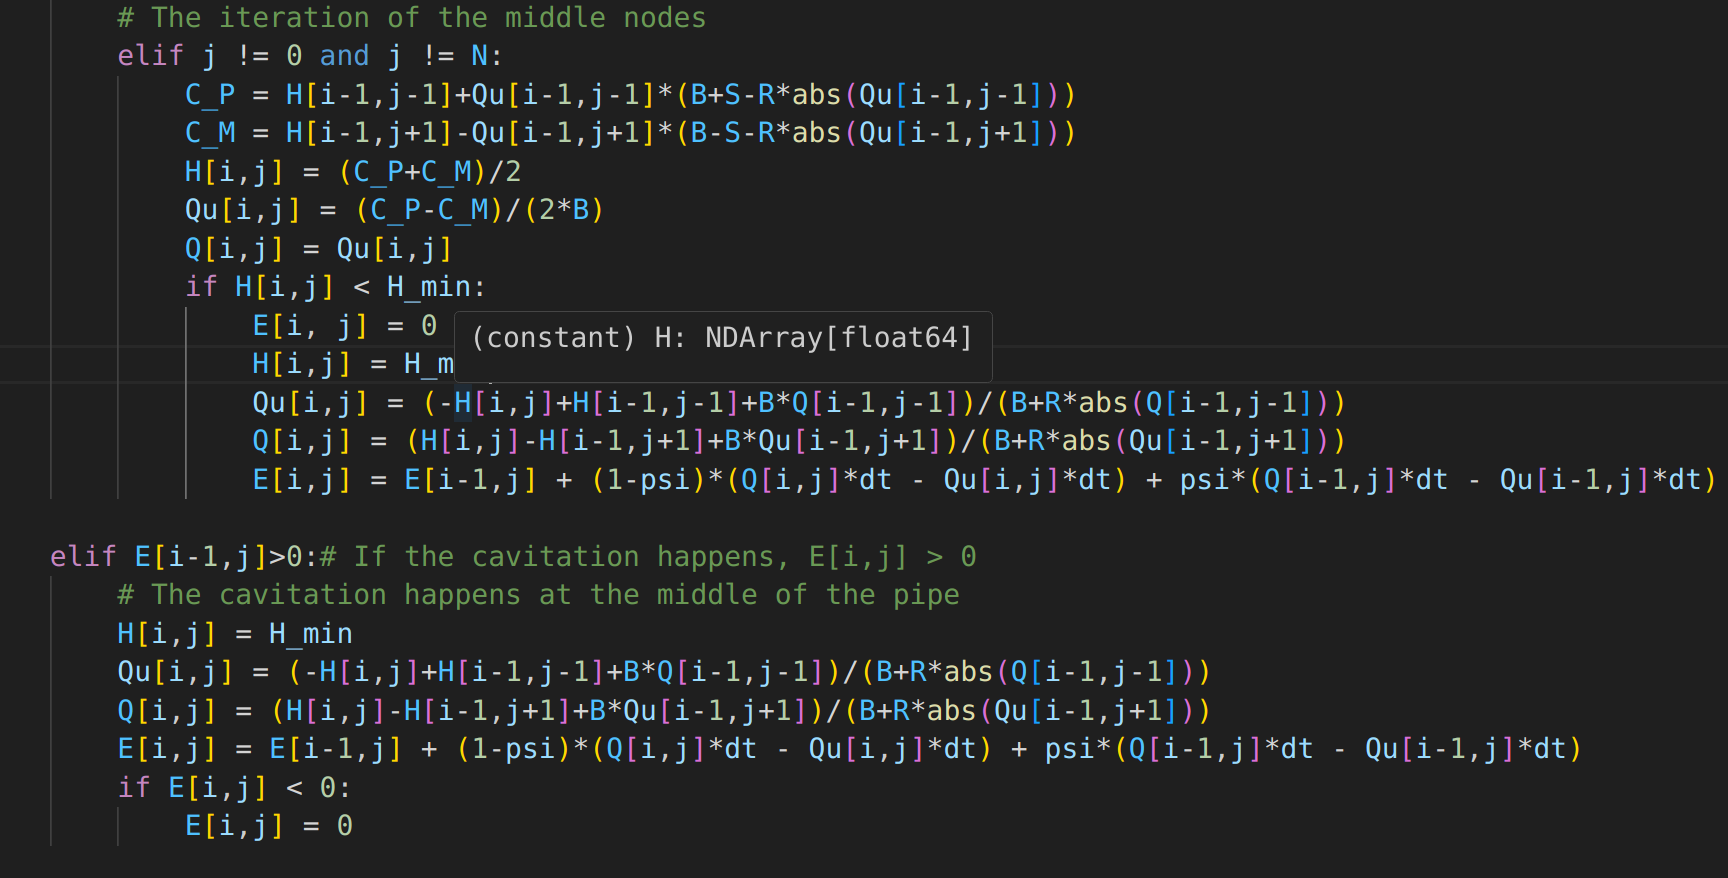
\includegraphics[width=0.8\textwidth]{pic/keycode.png}
        \caption{Key parts of the code to implement DVCM}
    \end{figure}
\end{frame}

\section{Results of DVCM}

\begin{frame}{Results of DVCM}
    \begin{figure}
        \centering
        % 将图片缩小到原来的0.8然后插入
        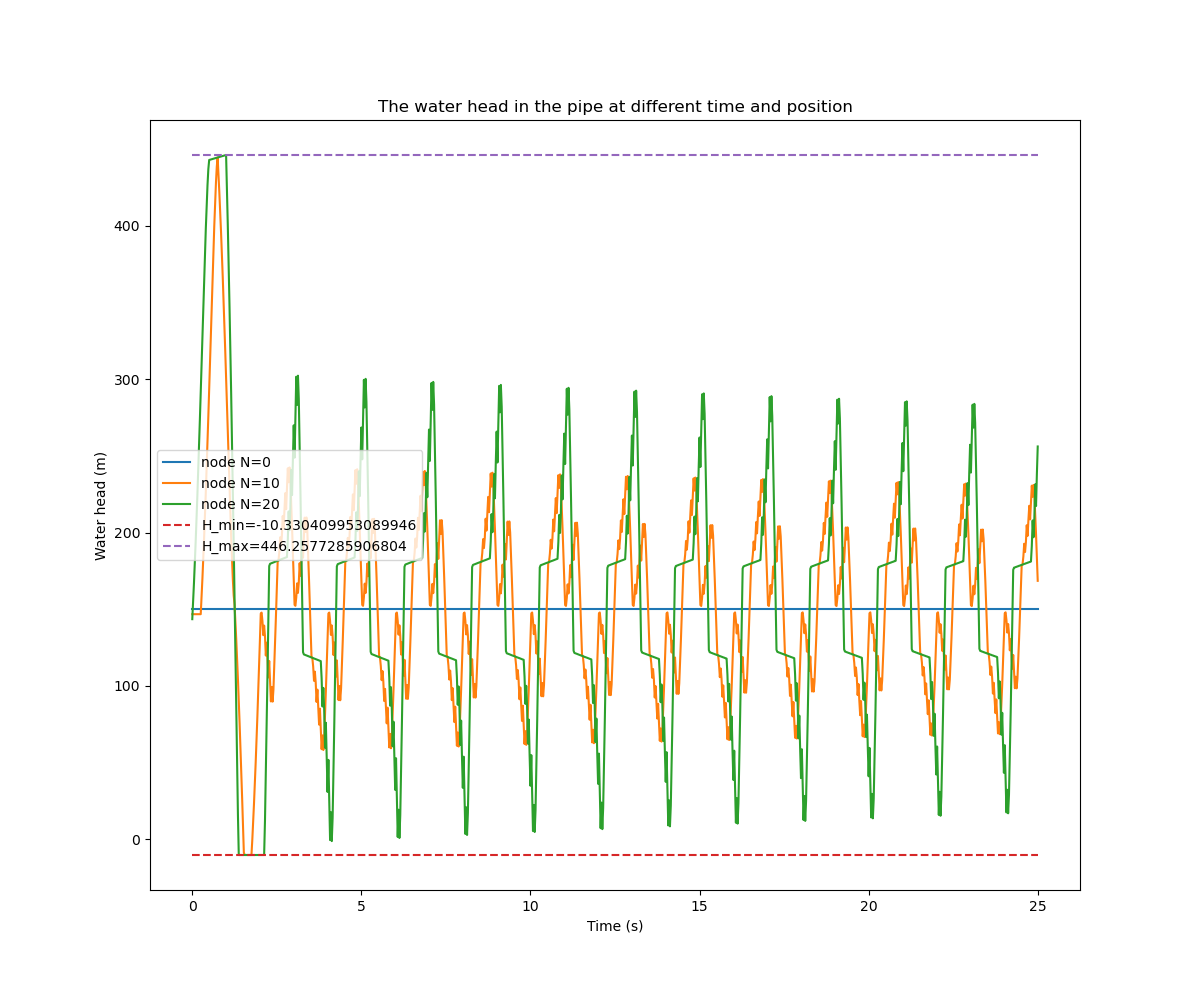
\includegraphics[width=0.8\textwidth]{pic/DVCM_Waterhead.png}
        \caption{Results of DVCM}
    \end{figure}
\end{frame}

\begin{frame}{Compared to Normal MOC}
    \begin{figure}
        \centering
        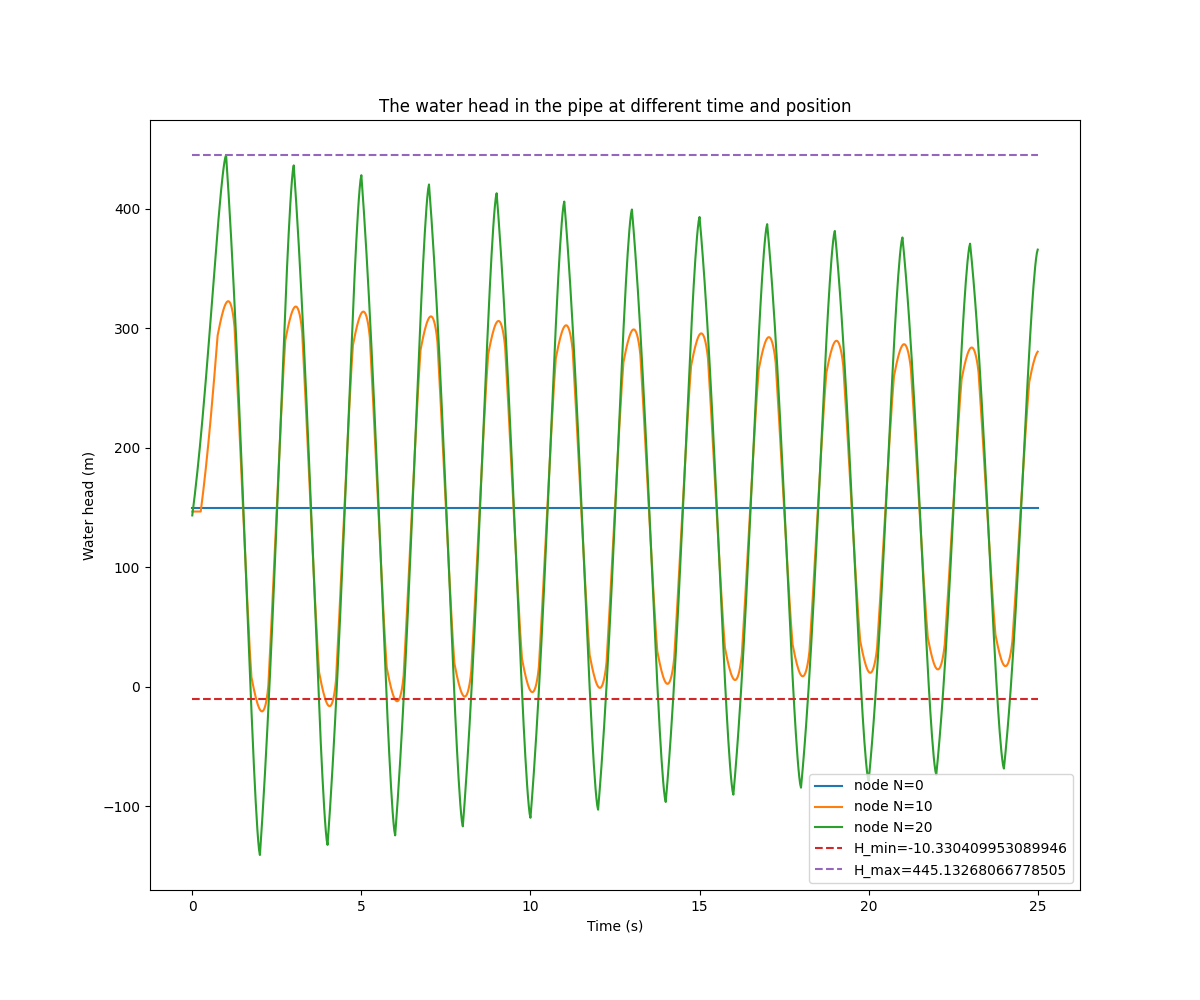
\includegraphics[width=0.8\textwidth]{pic/MOC_Waterhead.png}
        \caption{Results of MOC}
    \end{figure}
\end{frame}

\begin{frame}{Physics Features to Be Explained}
    \begin{itemize}
        \item The cavitation bubbles are generated and collapsed in the DVCM model so in some periods of time ,the pressure is a line with value $H^*$.
        \item The water head in the DVCM model is lower than the normal MOC model after the first oscillation. This could be explained that the generation and the diminishment of the cavitation bubbles consume the energy of the water.\\
        (Seems Good News? Less Pressure, Less Damage? Not Sure Yet!)
        \item The water head in the DVCM model is more fluctuated than the normal MOC model due to the turbulence of the cavitation bubbles.
    \end{itemize}
\end{frame}

\section{Future Work}

\begin{frame}{Future the Work}
    Congratulation: We have set the primary step on the moon!
    \begin{itemize}
        \item What do the experimenters say?
        \item Considering whether the DVCM can be developed by the conservation of mass and energy.
        \item What about other improved 1D models (DGCM discrete gas cavity model)?
        \item What about high dimensional models? Seems to be hard, limited desire to try. (QAQ)
    \end{itemize}
\end{frame}

\section{End}
\begin{frame}{Acknowledgement}
    \begin{itemize}
        \item Thanks to the teachers for the guidance.
        \item Thanks to the groupmates for their cooperation.
        \item Thanks to the audience for their attention.
        \item Thanks to Yuhan Zhang for her help.
    \end{itemize}
\end{frame}
\end{document}